\chapter{Fundamentos básicos}

\section{Leyes de \emph{Newton}}

\begin{itemize}
    \item Ley de Inercia.
    \item $F=ma$; $M_t=I\alpha$.
    \item Acción-Reacción.
\end{itemize}

\section{Energía cinética}

\begin{itemize}
    \item $T=\frac{1}{2}mv^2$.
    \item $T=\frac{1}{2}I\omega^2$.
\end{itemize}

\section{Transformaciones de coordenadas}

\subsection{Coordenadas polares}

\begin{figure}[H]
    \centering
    \includegraphics[scale=1.5]{resources/figura_01.eps}
    \caption{Coordenadas polares}\label{figura_01}
\end{figure}

\begin{equation*}
    \begin{cases}
        x=r\cos(\theta)\\
        y=r\sen(\theta)
    \end{cases}
\end{equation*}

\begin{equation*}
    T=\frac{1}{2}m(\dot{x}^2+\dot{y}^2)
\end{equation*}

Calculando la energía cinética en coordenadas polares:
n
\begin{equation*}
    \dot{x}=\dot{r}\cos(\theta)-r\sen(\theta)\dot{\theta}
\end{equation*}
\begin{equation*}
    \dot{y}=\dot{r}\sen(\theta)+r\cos(\theta)\dot{\theta}
\end{equation*}

\begin{equation*}
    \dot{x}^2=\dot{r}^2\cos^2(\theta)-
    2\dot{r}r\dot{\theta}\cos(\theta)\sen(\theta)+
    r^2\dot{\theta}^2\sen^2(\theta)
\end{equation*}
\begin{equation*}
    \dot{y}^2=\dot{r}^2\sen^2(\theta)+
    2\dot{r}r\dot{\theta}\sen(\theta)\cos(\theta)+
    r^2\dot{\theta}^2\cos^2(\theta)
\end{equation*}

\begin{equation*}
\begin{split}
    T&=\frac{1}{2}m(\dot{x}^2+\dot{y}^2)\\
     &=\frac{1}{2}m(\dot{r}^2\cos^2(\theta)+
       r^2\dot{\theta}^2\sen^2(\theta)+
       \dot{r}^2\sen^2(\theta)+
       r^2\dot{\theta}^2\cos^2(\theta))\\
     &=\frac{1}{2}m(\dot{r}^2(\cos^2(\theta)+
       \sen^2(\theta))+
       r^2\dot{\theta}^2(\sen^2(\theta)+
       \cos^2(\theta)))\\
     &=\frac{1}{2}m(\dot{r}^2+
       r^2\dot{\theta}^2)\\
\end{split}
\end{equation*}

\begin{equation}
\boxed{
    \begin{array}{l}
        T=\frac{1}{2}m(\dot{r}^2+r^2\dot{\theta}^2)
    \end{array}
}
\end{equation}

\subsection{Coordenadas cilíndricas}

\begin{figure}[H]
    \centering
    \includegraphics[scale=1.5]{resources/figura_02.eps}
    \caption{Coordenadas cilíndricas}\label{figura_02}
\end{figure}

\begin{equation*}
    \begin{cases}
        x=\rho\cos(\theta)\\
        y=\rho\sen(\theta)\\
        z=z
    \end{cases}
\end{equation*}

\begin{equation*}
    T=\frac{1}{2}m(\dot{x}^2+\dot{y}^2+\dot{z}^2)
\end{equation*}

Calculando la energía cinética en coordenadas cilíndricas:

\begin{equation*}
    \dot{x}=\dot{\rho}\cos(\theta)-\rho\sen(\theta)\dot{\theta}
\end{equation*}
\begin{equation*}
    \dot{y}=\dot{\rho}\sen(\theta)+\rho\cos(\theta)\dot{\theta}
\end{equation*}
\begin{equation*}
    \dot{z}=\dot{z}
\end{equation*}

\begin{equation*}
    \dot{x}^2=\dot{\rho}^2\cos^2(\theta)-
    2\dot{\rho}\rho\dot{\theta}\cos(\theta)\sen(\theta)+
    \rho^2\dot{\theta}^2\sen^2(\theta)
\end{equation*}
\begin{equation*}
    \dot{y}^2=\dot{\rho}^2\sen^2(\theta)+
    2\dot{\rho}\rho\dot{\theta}\sen(\theta)\cos(\theta)+
    \rho^2\dot{\theta}^2\cos^2(\theta)
\end{equation*}
\begin{equation*}
    \dot{z}^2=\dot{z}^2
\end{equation*}

\begin{equation*}
\begin{split}
    T&=\frac{1}{2}m(\dot{x}^2+\dot{y}^2+\dot{z}^2)\\
     &=\frac{1}{2}m(\dot{\rho}^2\cos^2(\theta)+
       \rho^2\dot{\theta}^2\sen^2(\theta)+
       \dot{\rho}^2\sen^2(\theta)+
       \rho^2\dot{\theta}^2\cos^2(\theta)+
       \dot{z}^2)\\
     &=\frac{1}{2}m(\dot{\rho}^2(\cos^2(\theta)+
       \sen^2(\theta))+
       \rho^2\dot{\theta}^2(\sen^2(\theta)+
       \cos^2(\theta))+
       \dot{z}^2)\\
     &=\frac{1}{2}m(\dot{\rho}^2+\rho^2\dot{\theta}^2+\dot{z}^2)\\
\end{split}
\end{equation*}

\begin{equation}
\boxed{
    \begin{array}{l}
        T=\frac{1}{2}m(\dot{\rho}^2+\rho^2\dot{\theta}^2+\dot{z}^2)
    \end{array}
}
\end{equation}

\subsection{Coordenadas esféricas}

\begin{figure}[H]
    \centering
    \includegraphics[scale=1.5]{resources/figura_03.eps}
    \caption{Coordenadas esféricas}\label{figura_03}
\end{figure}

\begin{equation*}
    \begin{cases}
        x=\rho\sen(\phi)\cos(\theta)\\
        y=\rho\sen(\phi)\sen(\theta)\\
        z=\rho\cos(\phi)
    \end{cases}
\end{equation*}

\begin{equation*}
    T=\frac{1}{2}m(\dot{x}^2+\dot{y}^2+\dot{z}^2)
\end{equation*}

Calculando la energía cinética en coordenadas esféricas:

\begin{equation*}
\begin{split}
    \dot{x}&=\dot{\rho}\sen(\phi)\cos(\theta)+
             \rho(\sen(\phi)\cos(\theta))'\\
           &=\dot{\rho}\sen(\phi)\cos(\theta)+
             \rho(\cos(\phi)\dot{\phi}\cos(\theta)+
             (-\sen(\theta))\dot{\theta}\sen(\phi))\\
           &=\dot{\rho}\sen(\phi)\cos(\theta)+
             \rho\dot{\phi}\cos(\phi)\cos(\theta)-
             \rho\dot{\theta}\sen(\theta)\sen(\phi)
\end{split}
\end{equation*}
\begin{equation*}
\begin{split}
    \dot{y}&=\dot{\rho}\sen(\phi)\sen(\theta)+
             \rho(\sen(\phi)\sen(\theta))'\\
           &=\dot{\rho}\sen(\phi)\sen(\theta)+
             \rho(\cos(\phi)\dot{\phi}\sen(\theta)+
             \cos(\theta)\dot{\theta}\sen(\phi))\\
           &=\dot{\rho}\sen(\phi)\sen(\theta)+
             \rho\dot{\phi}\cos(\phi)\sen(\theta)+
             \rho\dot{\theta}\cos(\theta)\sen(\phi)\\
\end{split}
\end{equation*}
\begin{equation*}
    \dot{z}=\dot{\rho}\cos(\phi)-\rho\dot{\phi}\sen(\phi)
\end{equation*}

\begin{equation*}
\begin{split}
    \dot{x}^2&=\dot{\rho}^2\sen^2(\phi)\cos^2(\theta)+
               \rho^2\dot{\phi}^2\cos^2(\phi)\cos^2(\theta)+
               \rho^2\dot{\theta}^2\sen^2(\theta)\sen^2(\phi)\\
             &+2\dot{\rho}\rho\dot{\phi}\sen(\phi)\cos^2(\theta)\cos(\phi)-
               2\rho^2\dot{\phi}\dot{\theta}
               \cos(\phi)\cos(\theta)\sen(\theta)\sen(\phi)-
               2\rho\dot{\rho}\dot{\theta}
               \sen^2(\phi)\cos(\theta)\sen(\theta)\\
\end{split}
\end{equation*}
\begin{equation*}
\begin{split}
    \dot{y}^2&=\dot{\rho}^2\sen^2(\phi)\sen^2(\theta)+
               \rho^2\dot{\phi}^2\cos^2(\phi)\sen^2(\theta)+
               \rho^2\dot{\theta}^2\cos^2(\theta)\sen^2(\phi)\\
             &+2\dot{\rho}\rho\dot{\phi}\sen(\phi)\sen^2(\theta)\cos(\phi)+
               2\rho^2\dot{\phi}\dot{\theta}
               \cos(\phi)\sen(\theta)\cos(\theta)\sen(\phi)+
               2\rho\dot{\theta}\dot{\rho}
               \cos(\theta)\sen^2(\phi)\sen(\theta)
\end{split}
\end{equation*}
\begin{equation*}
    \dot{z}^2=\dot{\rho}^2\cos^2(\phi)-
              2\dot{\rho}\rho\dot{\phi}\cos(\phi)\sen(\phi)+
              \rho^2\dot{\phi}^2\sen^2(\phi)
\end{equation*}

\begin{equation*}
\begin{split}
    T&=\frac{1}{2}m(\dot{x}^2+\dot{y}^2+\dot{z}^2)\\
     &=\frac{1}{2}m(\dot{\rho}^2\sen^2(\phi)+
       \rho^2\dot{\phi}^2\cos^2(\phi)+
       \rho^2\dot{\theta}^2\sen^2(\phi)\\
     &+2\dot{\rho}\rho\dot{\phi}\sen(\phi)\cos(\phi)+
       \dot{\rho}^2\cos^2(\phi)-
       2\dot{\rho}\rho\dot{\phi}\cos(\phi)\sen(\phi)+
       \rho^2\dot{\phi}^2\sen^2(\phi))\\
     &=\frac{1}{2}m(\dot{\rho}^2+
       \rho^2\dot{\phi}^2+
       \rho^2\dot{\theta}^2\sen^2(\phi))
\end{split}
\end{equation*}

\begin{equation}
\boxed{
    \begin{array}{l}
        T=\frac{1}{2}m(\dot{\rho}^2+
        \rho^2\dot{\phi}^2+
        \rho^2\dot{\theta}^2\sen^2(\phi))
    \end{array}
}
\end{equation}

